\section{Utilisation type}
Dans cette partie sera évoqué une description du processus de fonctionnement du programme.

\subsection{Lancement de l'application Androïd}

\paragraph{Captation d'un unique ouvrage} 


Si l'utilisateur choisi le mode de captation unique, alors le programme vérifie si l'adresse mail est configurée ou non. 
Si elle ne l'est pas, alors le programme lance le processus de configuration de l'email. 
Une fois certain que l'adresse email est correctement configurée, la phase de capture réelle est exécutée. 
Si l'\emph{ISBN} retourné est valide, alors nous envoyons les informations sur le client PC. 
Si ça n'est pas le cas, alors on proposera à l'utilisateur de refaire une capture. 


\begin{figure}[htbp]
  \begin{center}
    \leavevmode
    \subfloat[Menu de l'application Royal\_Scanner]{%
		\label{}
		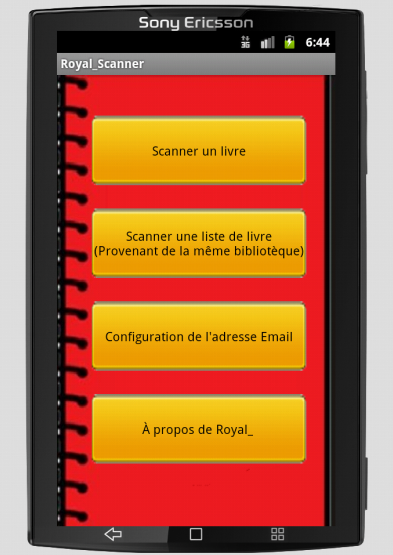
\includegraphics[height=7cm]{../img/Royal_Scanner_menu.png}}
    \hspace{4cm}
    \subfloat[Phase de capture du code barre]{%
		\label{}
		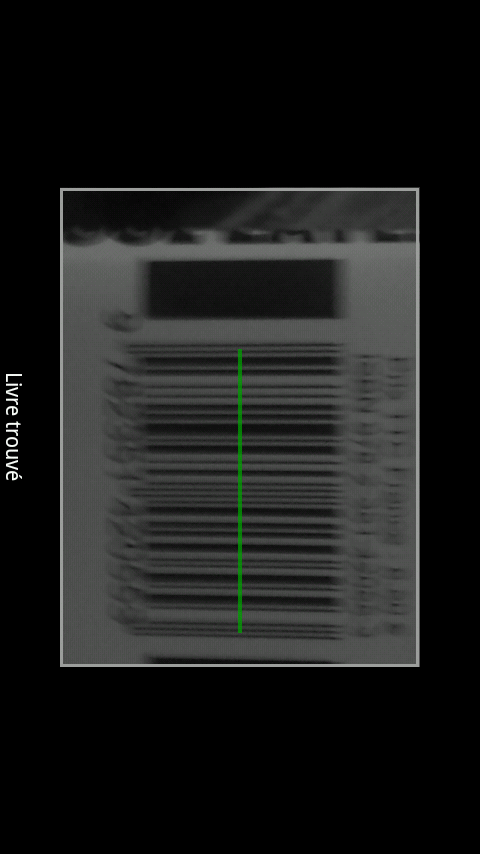
\includegraphics[height=7cm]{../img/Royal_Scanner_prisescanner_2.png}}
  \end{center}
\end{figure}

%Lancement de l'application Androïd
%	Captation Unique 
%		Si adresse mail non configurée 
%			Alors lancement de la configuration du mail
%		Lancement de la phase de captation
%		Vérification de la validité 
%		Si valide 
%			Alors envois 
%		Si non 
%			Propotition de recaptation 
\paragraph{Capture d'un lot d'ouvrages}
Si l'utilisateur choisi de capturer directement plusieurs BD, alors le programme exécutera en boucle le processus utilisé pour une simple \emph{bd}. 
Le seul changement interviendra après la validation de la bonne captation de l'\emph{ISBN} :
Il sera en effet demandé à l'utilisateur si celui-ci désire continuer la capture ou y prendre fin. 

Si il choisi d'y prendre fin, alors les informations seront transmises au client PC. 
Si au contraire, il choisi de continuer la capture, alors le programme rebouclera. 

%		Similaire à la captation unique exepté phase de validation 
%		Si valide 
%			Alors proposition d'une captation supplémentaire 
%			Si fin 
%				Alors envois des informations sur les livres 


\subsection{Lancement de l'application PC}


\begin{wrapfigure}[5]{r}[1cm]{5cm}
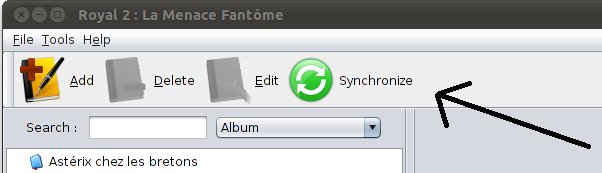
\includegraphics[width=5cm]{../img/btn_synchro.png}
\caption{Boutton de l'importation}
\end{wrapfigure}
\paragraph{Importation des livres}
Si l'utilisateur choisi d'importer les livres. Alors le programme teste si l'adresse email est correctement configurée. Si ce n'est pas le cas, le processus de configuration est exécuté. 

Une fois que le programme a une configuration d'email valide, celui-ci recherche sur la boite email si des messages sont présents à son attention. 

\begin{wrapfigure}[12]{r}[1.5cm]{8cm}
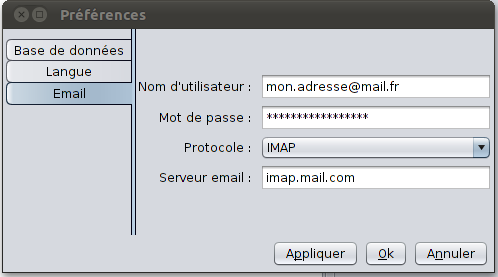
\includegraphics[width=8cm]{../img/preferenceMail.png}
\caption{Configue du mail}
\end{wrapfigure}
\paragraph{Importation des livres}
Si c'est le cas, alors la récupération à lieu. 
Tant qu'il y a des messages à l'attention du programme, celui-ci les lis. 
Tant que des numéro d'\emph{ISBN} sont présents dans le mail, ils sont récupérés. 
Une fois tout les \emph{ISBN} récupérés, le programme recherche des informations sur les livres sur internet.
L'utilisateur peut ensuite modifier ses données, puis peut renseigner les informations relatives à la bibliothèque. 

Si la bibliothèque dans la quelle le livre (ou le lot) a été emprunté existe déjà, 
alors l'utilisateur n'aura qu'à le choisir dans une liste. Si elle n'existe pas encore, elle pourra être rajouté via une fonction disponible. 
Enfin, l'utilisateur pourra indiquer la date de retour maximale du livre (ou du lot).

\paragraph{Vérification de la date de retour}
À chaque lancement de programme, les dates de tous les ouvrages encore en possetion de l'utilisateur seront testé afin de voir si l'ultimatum restant est plus petit que la valeur fixé par l'utilisateur après le quel un rappel doit être effectué. 
Si l'ultimatum est plus petit pour un livre, son nom est stocké en mémoire. 
Les noms de tous les livres ainsi repérés sont conservés puis affichés à l'utilisateur une fois la recherche terminée. 

%Lancement de l'application PC 
%	Si importation 
%		Alors si adresse mail non configuré 
%			Alors configuration de l'adresse mail 
%		Récupération des mails 
%			Si des mails sont récupérés 
%				Alors ajout des albums uniques ou par lot, automatique dans l'application avec possibilité d'ajout d'une bibliothèque et d'une date de retour. 

\begin{wrapfigure}[10]{l}[1cm]{8cm}
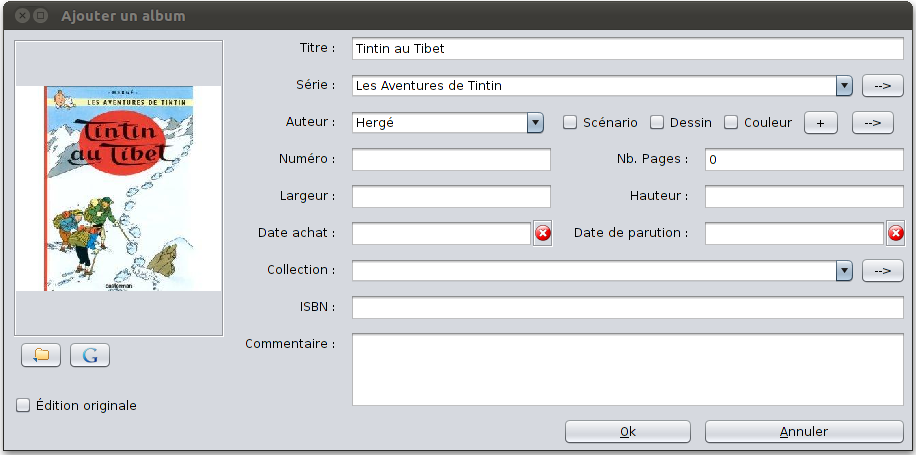
\includegraphics[width=8cm]{../img/editionAlbum.png}
\caption{Edition d'un Album}
\end{wrapfigure}
\paragraph{Modification des information d'un livre}
Si l'utilisateur souhaite modifier des information sur un livre enregistré dans le programme, il pourra visualiser les album par critere tels que l'auteur, la collection, le type...
Une fois son livre selectionné en cliquant sur le boutton editer l'utilisateur verra apparaitre les différentes informations sur le livre et pourra les modifier.
Une fois les information modifié l'utilisateur pourra soit valider les modification éfféctué soit les annuler. 
En cas de validation de la modification le programme enregistrera les nouvelle information dans la base de données.  
